\chapter{Preliminary results and planning}
\label{chapter:preliminary_results}

\section{Preliminary results}

To get a better understanding of the GGP platform, a few tests were run, using the application \textit{Kiosk} as a game manager (provided by ggp.org) and a few different game players:

\begin{itemize}

\item Sancho

\item Example MCTS+UCT player with Propositional Networks (tried different exploration bias values)

\item Example MCTS+UCT player with a Prolog reasoner

\item Example Mini-Max player with Alpha-Beta prunning and a Prolog reasoner

\item Example Mini-Max player without Alpha-Beta prunning and a Prolog reasoner

\item Example random legal player

\item A few other small variations of the example players, like enabling state caching on all of them.

\end{itemize}

Games on the \textit{Kiosk} application have graphical user interfaces and even allow a user to play directly against a player.
A few of the tested players were created by mixing and matching different software components already provided by ggp.org.

Overall, it was quite useful to get some practical knowledge on the field but performance comparisons proved to be quite laborious (many different games have to be tested for the results to have meaning) and so were avoided since better options already exist, namely the Tiltyard game server. Even so, in the small sample of games tested, Sancho was noticeably much better than the example players and myself, remaining unbeaten in games where it didn't run out of RAM (it was running on a machine with 6GB of RAM versus the 32GB it runs on for competitions).

\section{Planning}

\subsection{Work proposal}
From the research made in chapter \ref{chapter:state_of_the_art} it seems the most significant ways to advance \gls{GGP} research is to develop improvements to Propositional Network techniques and/or run-time creation of heuristics based on game rule analysis and so these will be the focus of the dissertation.

\subsection{Objectives and timeline}

\begin{table}[h]
\caption{Planned dates for the objectives}
\label{table:Planning}
\small
%\begin{tabular}{| c | p{1cm} | p{2.5cm} | p{2.5cm} | p{2.8cm} | c | p{2.2cm} |}
\begin{tabular}{| c | c | c |}
\hline Primary objectives & Start date & End date \\

\hline Research and compare current techniques and solutions for GGP players & 18/Jan/2016 & 14/Feb/2016 \\
\hline Improve or develop new techniques for game playing & 01/Feb/2016 & 10/Apr/2016 \\
\hline Use the improvements to make a new GGP player & 11/Apr/2016 & 22/May/2016 \\
\hline Benchmark the player against other existing GGP players & 23/May/2016 & 12/Jun/2016 \\

\hline Secondary objectives & Start date & End date \\

\hline Publish the results & 20/Jun/2016 & 17/Jul/2016 \\
\hline Take the online course on GGP & 28/Mar/2016 & 17/Jul/2016 \\
\hline Enter the annual GGP competition & 06/Jun/2016 & 15/Jun/2016 \\
\hline Enter other relevant competitions & - & - \\

\hline
\end{tabular}
\end{table}


\begin{figure}[h]
	\centering
    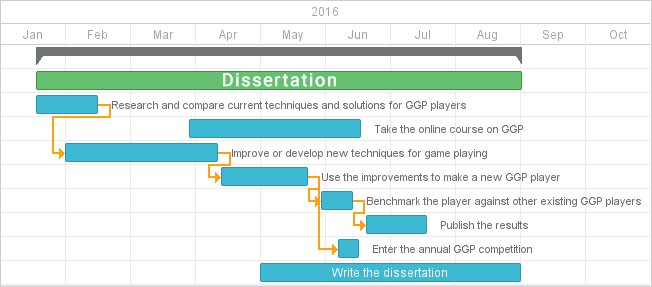
\includegraphics[scale=0.6]{images/gantt.png}
    \caption{Gantt chart for the dissertation}
    \label{fig:gantt}
\end{figure}
